\section{System Design}
	\hspace{10mm}This section will detail the design of my Logging Aggregator System. To better illustrate the network, I'll start with a image:\\
	
	\begin{figure}[h!]
		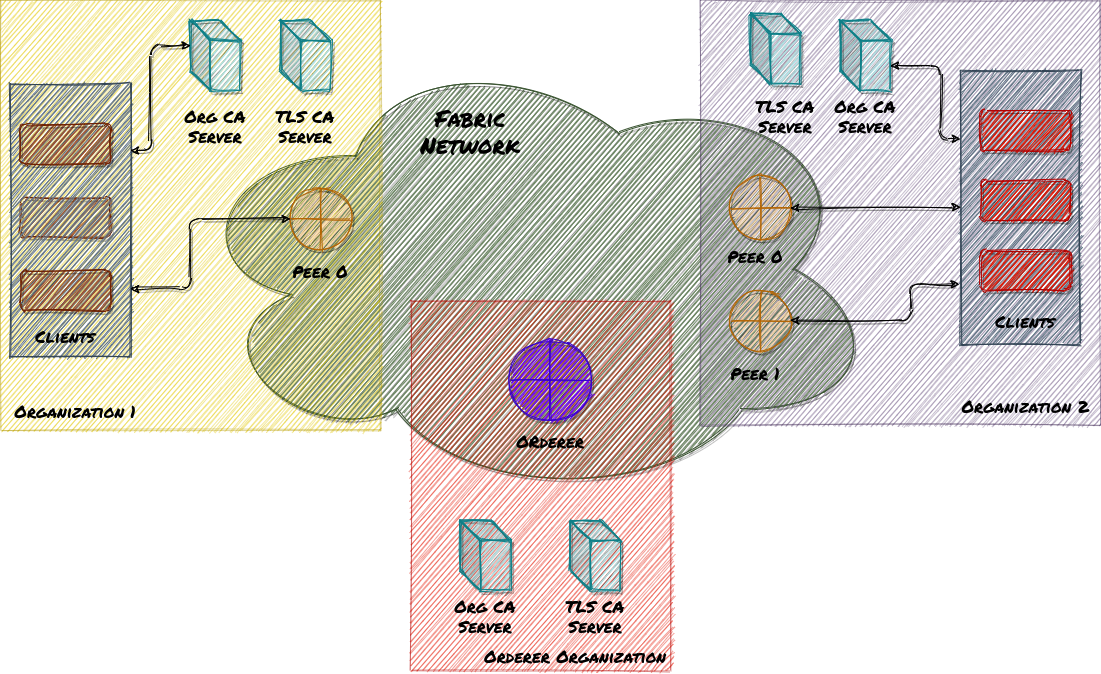
\includegraphics[width=\textwidth]{./fabsec-report-system-design/fabric-network-diagram.png}
		\caption{The FabSec Network Topography}
	\end{figure}
	
	\hspace{10mm}At a high level this system will have three Organizations involved: two Peer Organizations and an Orderer Organization. The Peer Organizations will be the participants that will effective be the users of the system. In the context of the Log Aggregator network, they will be the ones collecting the log messages to send to the Orderer as messages in the transactions, and they are responsible for retrieving those message back at the appropriate time. The Orderer Organization acts as the consensus nodes. It will do the assembling of transactions into blocks, validates those transactions/blocks, and finally disseminates the blocks to the peers. Since this is a distributed network, the Orderer will be a "third-party" outside of those that are peers to a particular Channel.\\
	
	\hspace{10mm}The following is a directory listing view of how the structure for this project will look:
	
	\verbatiminput{./fabsec-report-system-design/fabsec-org-tree-nonuni.txt}
	
	\hspace{10mm}Note: To save space, this is not the entire listing with all of the different files that are needed to make the system work. However, it is a good guide illustration of the general structure of not only how it looks for, say, a node like orderer0.org0.fabsec.com vs an organization like org0.fabsec.com, but how the organizations are logically separated.\\
	
	\hspace{10mm}There will be a dedicated TLS CA and a dedicated Fabric CA for each Organization. This choice is to reflect a real-world scenario where geographically separated Organizations will have their own set of CAs. Speaking of CAs, while it is an option to deploy intermediate CAs (and a solid security decision to do so) for scalability, this project won't be using any. Another decision made in dealing with CA is that of credentials. Credentials, i.e. username and password, are used when register and enrolling entities that will eventually become identities. For now, I have made these static within the scripts that help fire up the network, however a future consideration would be to make them dynamic, allowing a script operator to feed them as commandline arguments to the script.\\
	
	\hspace{10mm}There are two options for, what's called, the State Database: CouchDB and LevelDB. The State Database is a database maintained by each Peer node and presents an indexed view of the current values for all of the assets on the Ledger. While a deep dive into this database is outside the scope of this project, let it be said that LevelDB is the default, and embedded, choice for this decision and the one used for this project.
	
	\hspace{10mm}Port management is a bit of a nightmare here. In a real world system, this will not be as hectic as an Organization will likely be running all of the nodes on separate physical machines. However, for this project, I'm hardcoded the ports that all of the different entities will run on. They are as follows:
		\begin{itemize}
			\item Org0, TLS CA -- main: 7054, operations: 9443
			\item Org0, Fab CA -- main: 7055, operations: 9444
			\item Org0, orderer0 -- main: 6050, operations: 8443
			\item Org1, TLS CA -- main: 7056, operations: 9445
			\item Org1, Fab CA -- main: 7057, operations: 9446
			\item Org1, peer0 -- main: 6051, chaincode: 6052, operations: 8446			
			\item Org2, TLS CA -- main: 7058, operations: 9447
			\item Org2, Fab CA -- main: 7059, operations: 9448
			\item Org2, peer0 -- main: 6053, chaincode: 6054, operations: 8447
			\item Org2, peer1 -- main: 6055, chaincode: 6056, operations: 8448
		\end{itemize}